\documentclass{webofc}
\usepackage[varg]{txfonts}
\usepackage{xspace}
\usepackage{hyperref}

\newcommand{\ctau}[0]{\ensuremath{c\tau_{0}}\xspace}

\begin{document}

\title{Identification of new long-lived particles using deep neural networks}

\author{\firstname{Matthias} \lastname{Komm} \inst{1}\fnsep\thanks{\email{Matthias.Komm@cern.ch}}, for the CMS Collaboration}

\institute{Imperial College London, Physics Department, SW7 2BW London, United Kingdom}

\abstract{
We present the development of a deep neural network for identifying generic displaced jets arising from the decays of new long-lived particles in data recorded by the CMS detector at the CERN LHC. Various jet features including detailed information about each clustered candidate as well as reconstructed secondary vertices are refined through the use of 1-dimensional convolution layers before being combined with high-level engineered features and passed through a series of fully-connected layers. The lifetime, $\tau_{0}$, is treated as a parameter of the neural network model, which allows for hypothesis testing over several orders of magnitude ranging from $\ctau = 1\,\mu\textrm{m}$ to 10\,m. Domain adaptation by backward propagation is performed using data to construct domain-independent features at an intermediate layer of the network. The training is performed by streaming ROOT trees containing $\mathcal{O}$(100M) jets directly into the TensorFlow queue and threading system allows a flexible selection of input features and the asynchronous preprocessing of data, such as the resampling and shuffling of batches on the CPU, in parallel to training on the GPU. The performance of the tagger is demonstrated in a search for long-lived gluinos as predicted by split supersymmetric models.
}

\maketitle
%
\section{Introduction}
\label{intro}

Machine-learned algorithms are routinely deployed to perform event reconstruction, particle identification, event classification, and other tasks~\cite{ml-white-paper} when analysing data samples recorded by experiments at the CERN LHC. For example, the ATLAS~\cite{atlas} and CMS~\cite{cms} Collaborations have developed numerous algorithms based on boosted decision trees or neural networks to identify jets originating from the hadronisation of bottom quarks with unprecedented performance~\cite{batlas,bcms}.

In this note, the development and application of a novel algorithm is presented for identifying jets originating from the decay of long-lived particles. It is based on a deep neural network (DNN) that is inspired by the CMS DeepJet approach~\cite{} albeit several aspects require an extension of the established architecture and training procedure. First, to perform supervised learning a generic definition for displaced jets is introduced. Secondly, the DNN is parametrised as a function of the proper lifetime, $\tau_{0}$, of the long-lived particle to allow hypothesis testing over a broad range of scenarios. Uncertainties arising from difference between data and simulation are mitigated by incorporating domain adaptation by backward propagation.
The application of the tagger is demonstrated in a search for long-lived gluino production as predicted by split supersymmetric (SUSY) models.

This note is based on Ref.~\cite{CMS-EXO-19-011}.

\section{Simulated samples and jet labelling}
\label{sec-1}


\begin{figure*}[!ht]
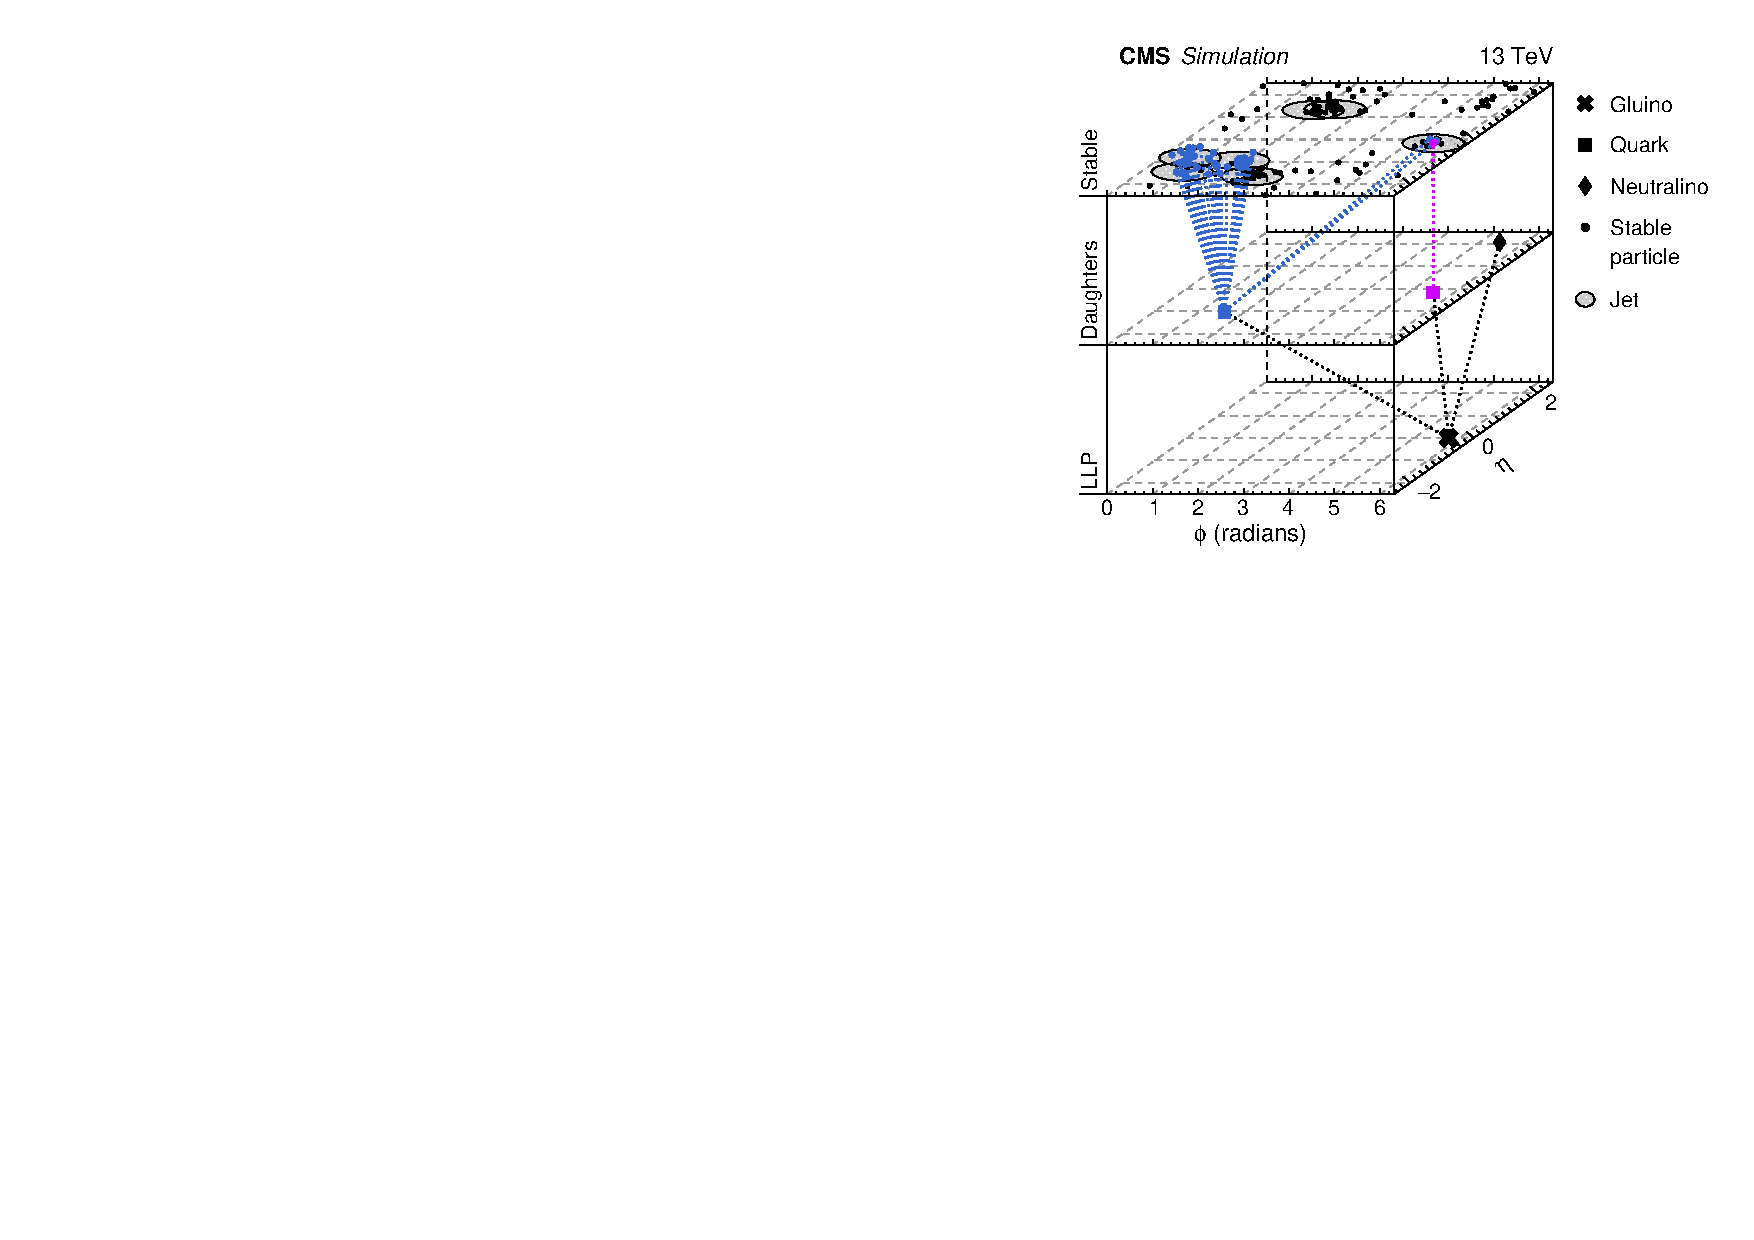
\includegraphics[width=0.48\textwidth]{figs/decay1.pdf}\hspace{0.03\textwidth}
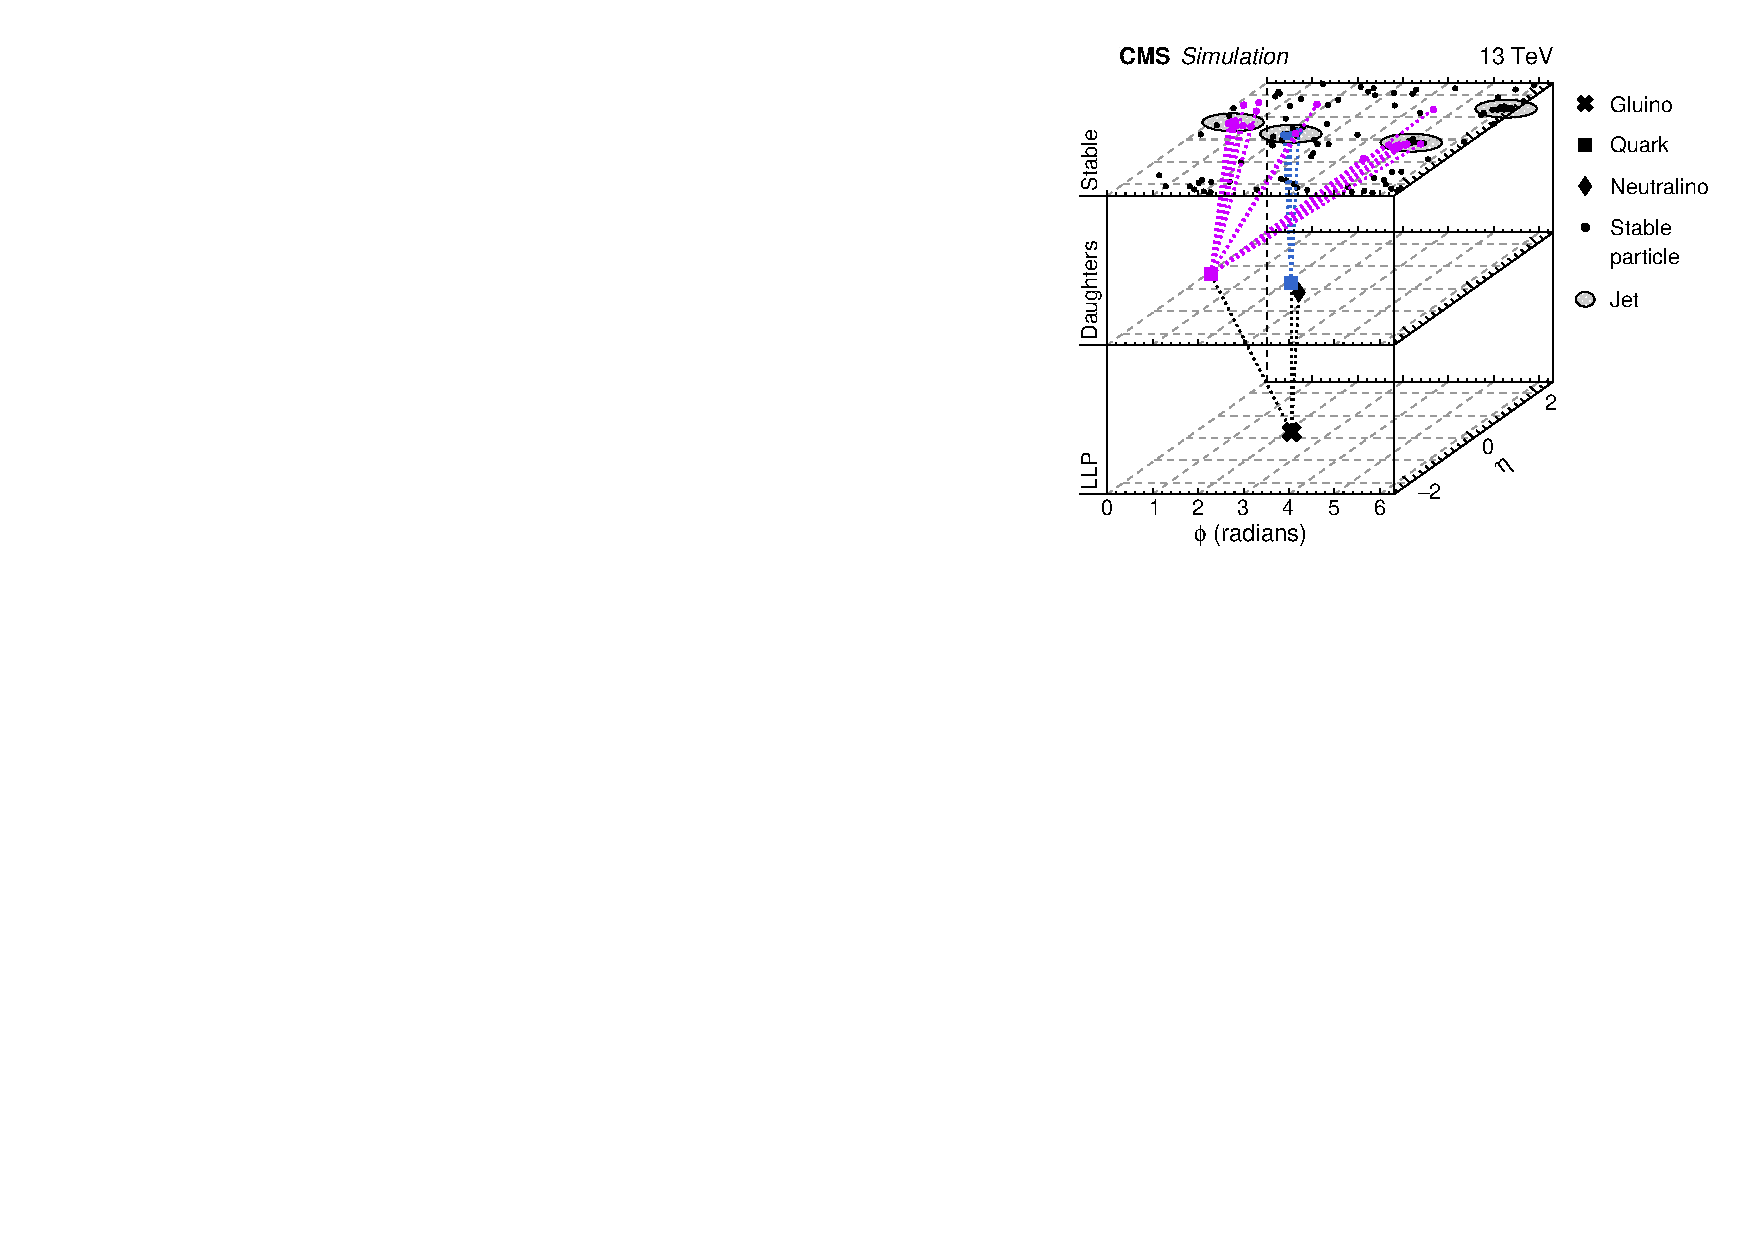
\includegraphics[width=0.48\textwidth]{figs/decay2.pdf}
\centering
\caption{The figures are taken from Ref.~\cite{CMS-EXO-19-011}.}
\label{fig-1}
\end{figure*}


\section{Neural network architecture and training}
\label{sec-2}
Don't forget to give each section, subsection, subsubsection, and
paragraph a unique label (see Sect.~\ref{sec-1}).

For two-column wide figures use syntax of figure~\ref{fig-2}

\begin{figure*}[!ht]
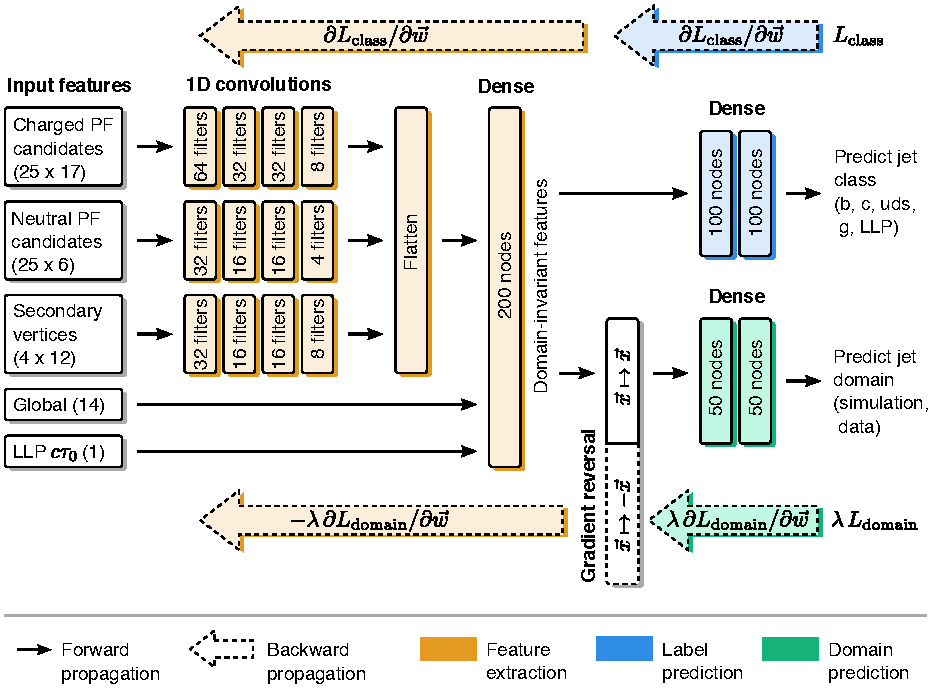
\includegraphics[width=0.9\textwidth]{figs/network.pdf}
\centering
\caption{The figure is taken from Ref.~\cite{CMS-EXO-19-011}.}
\label{fig-2}
\end{figure*}

\begin{figure*}[!ht]
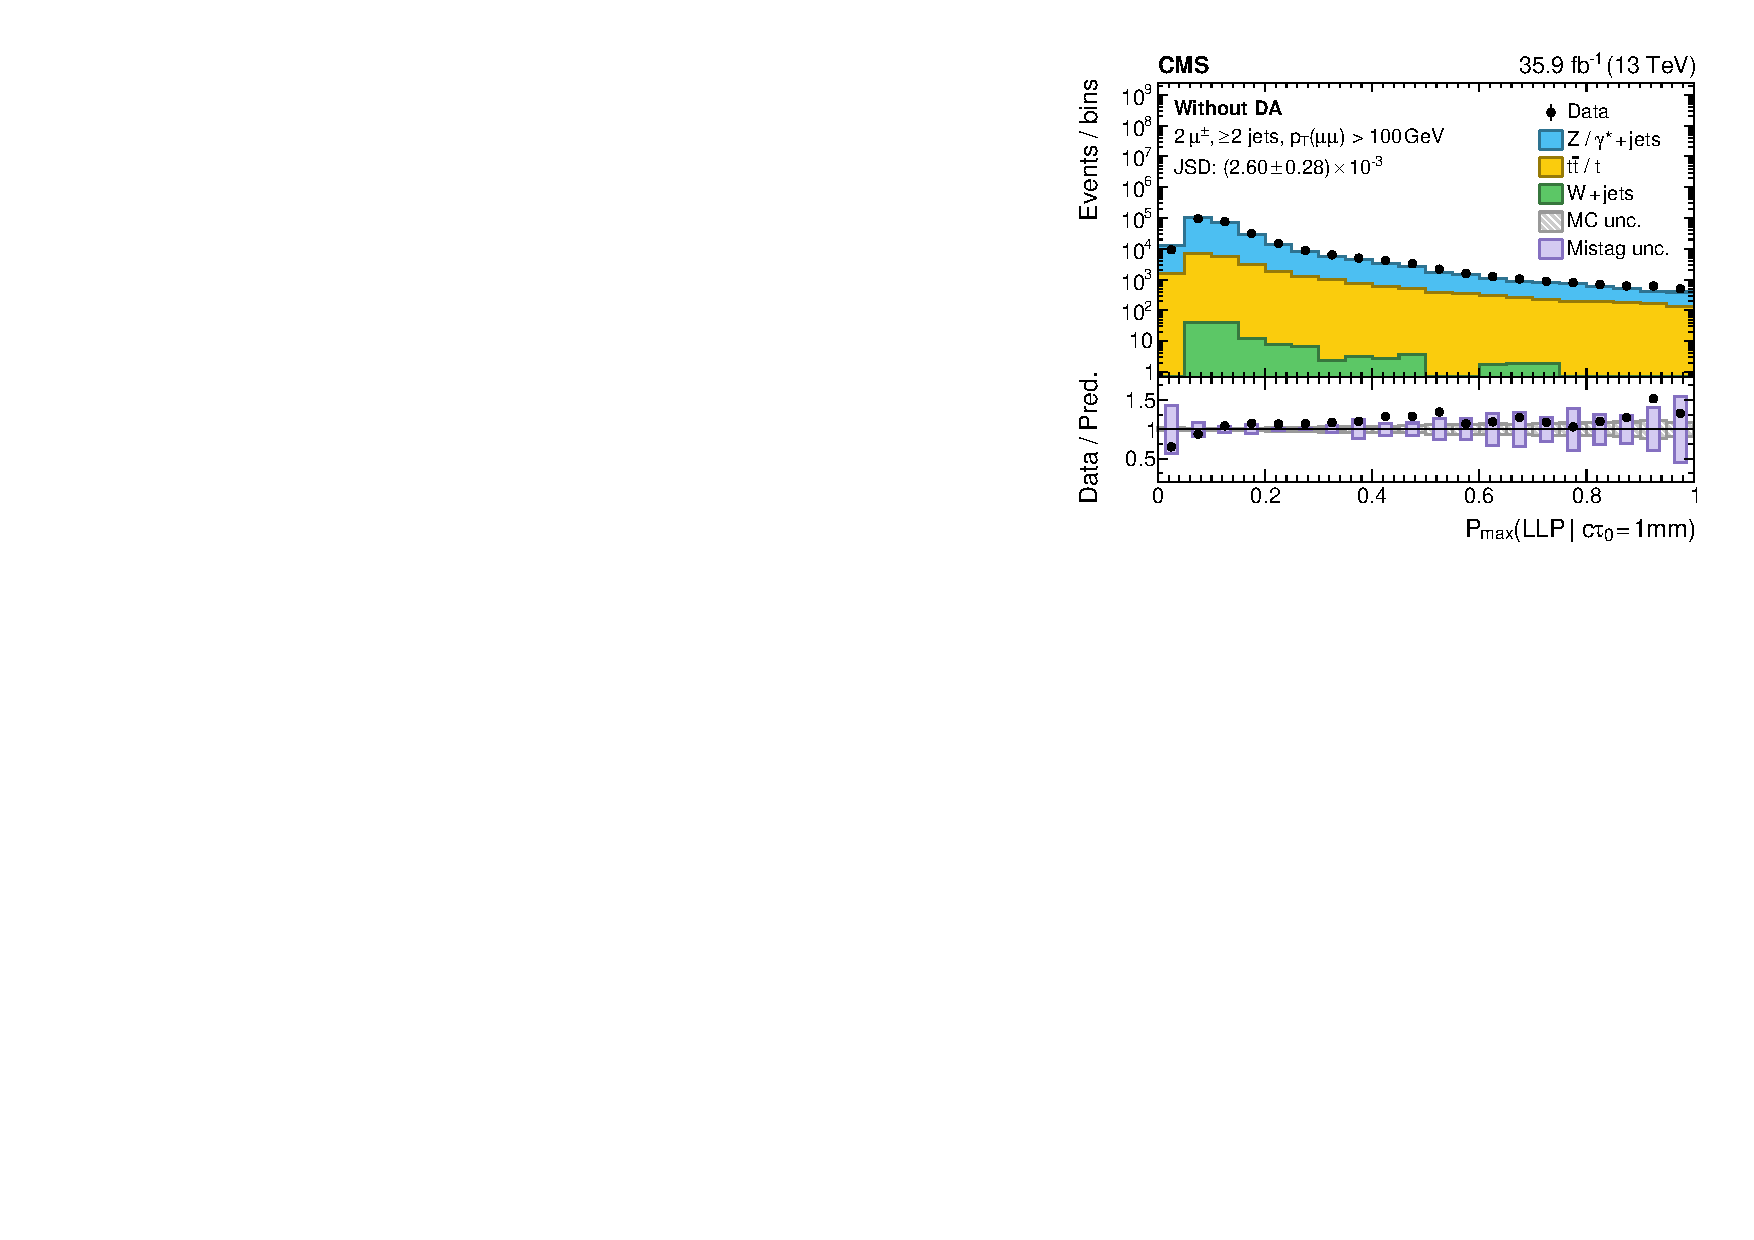
\includegraphics[width=0.48\textwidth]{figs/2mu_2toNj__llpdnnx_noda_0_max_highpt.pdf}\hspace{0.03\textwidth}
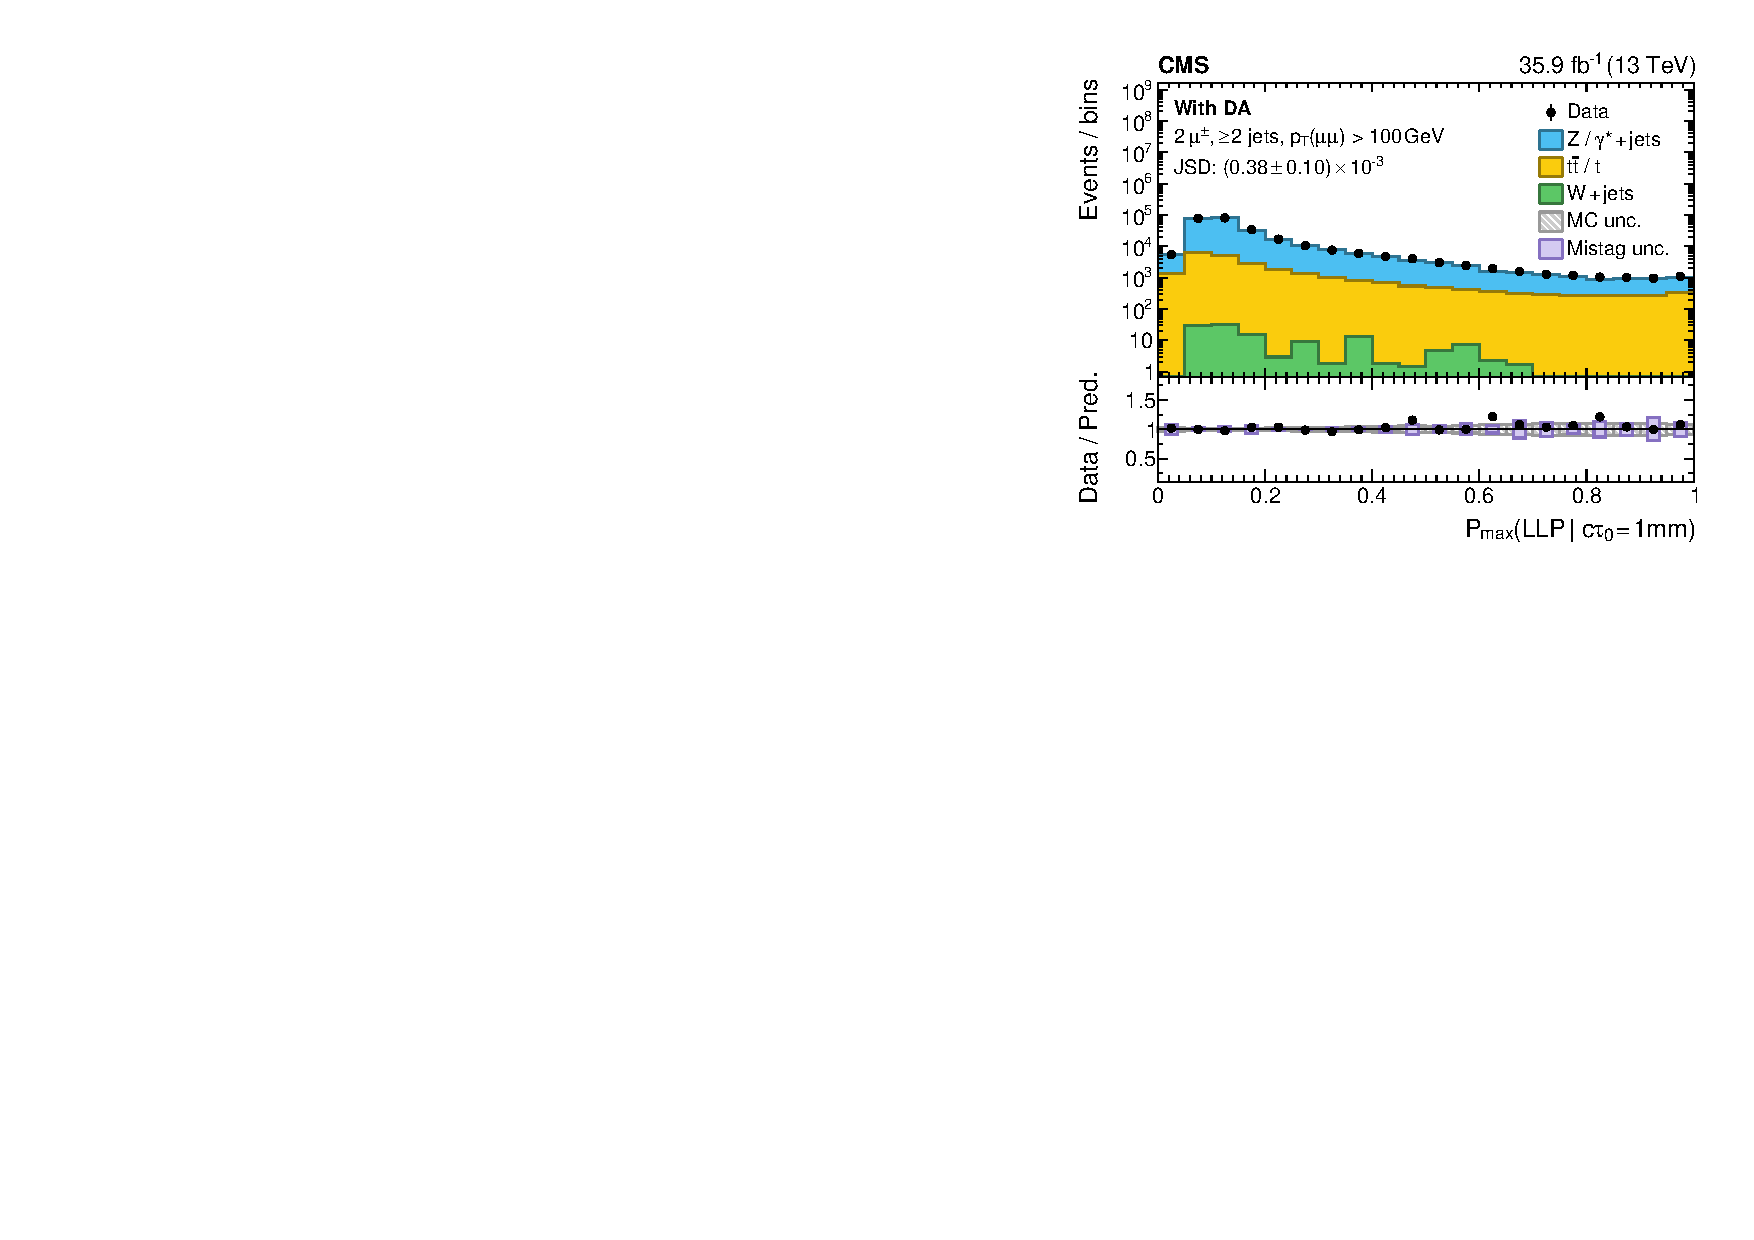
\includegraphics[width=0.48\textwidth]{figs/2mu_2toNj__llpdnnx_da_0_max_highpt.pdf}
\centering
\caption{The figures are taken from Ref.~\cite{CMS-EXO-19-011}.}
\label{fig-3}
\end{figure*}

\section{Performance}

\begin{figure*}[!ht]
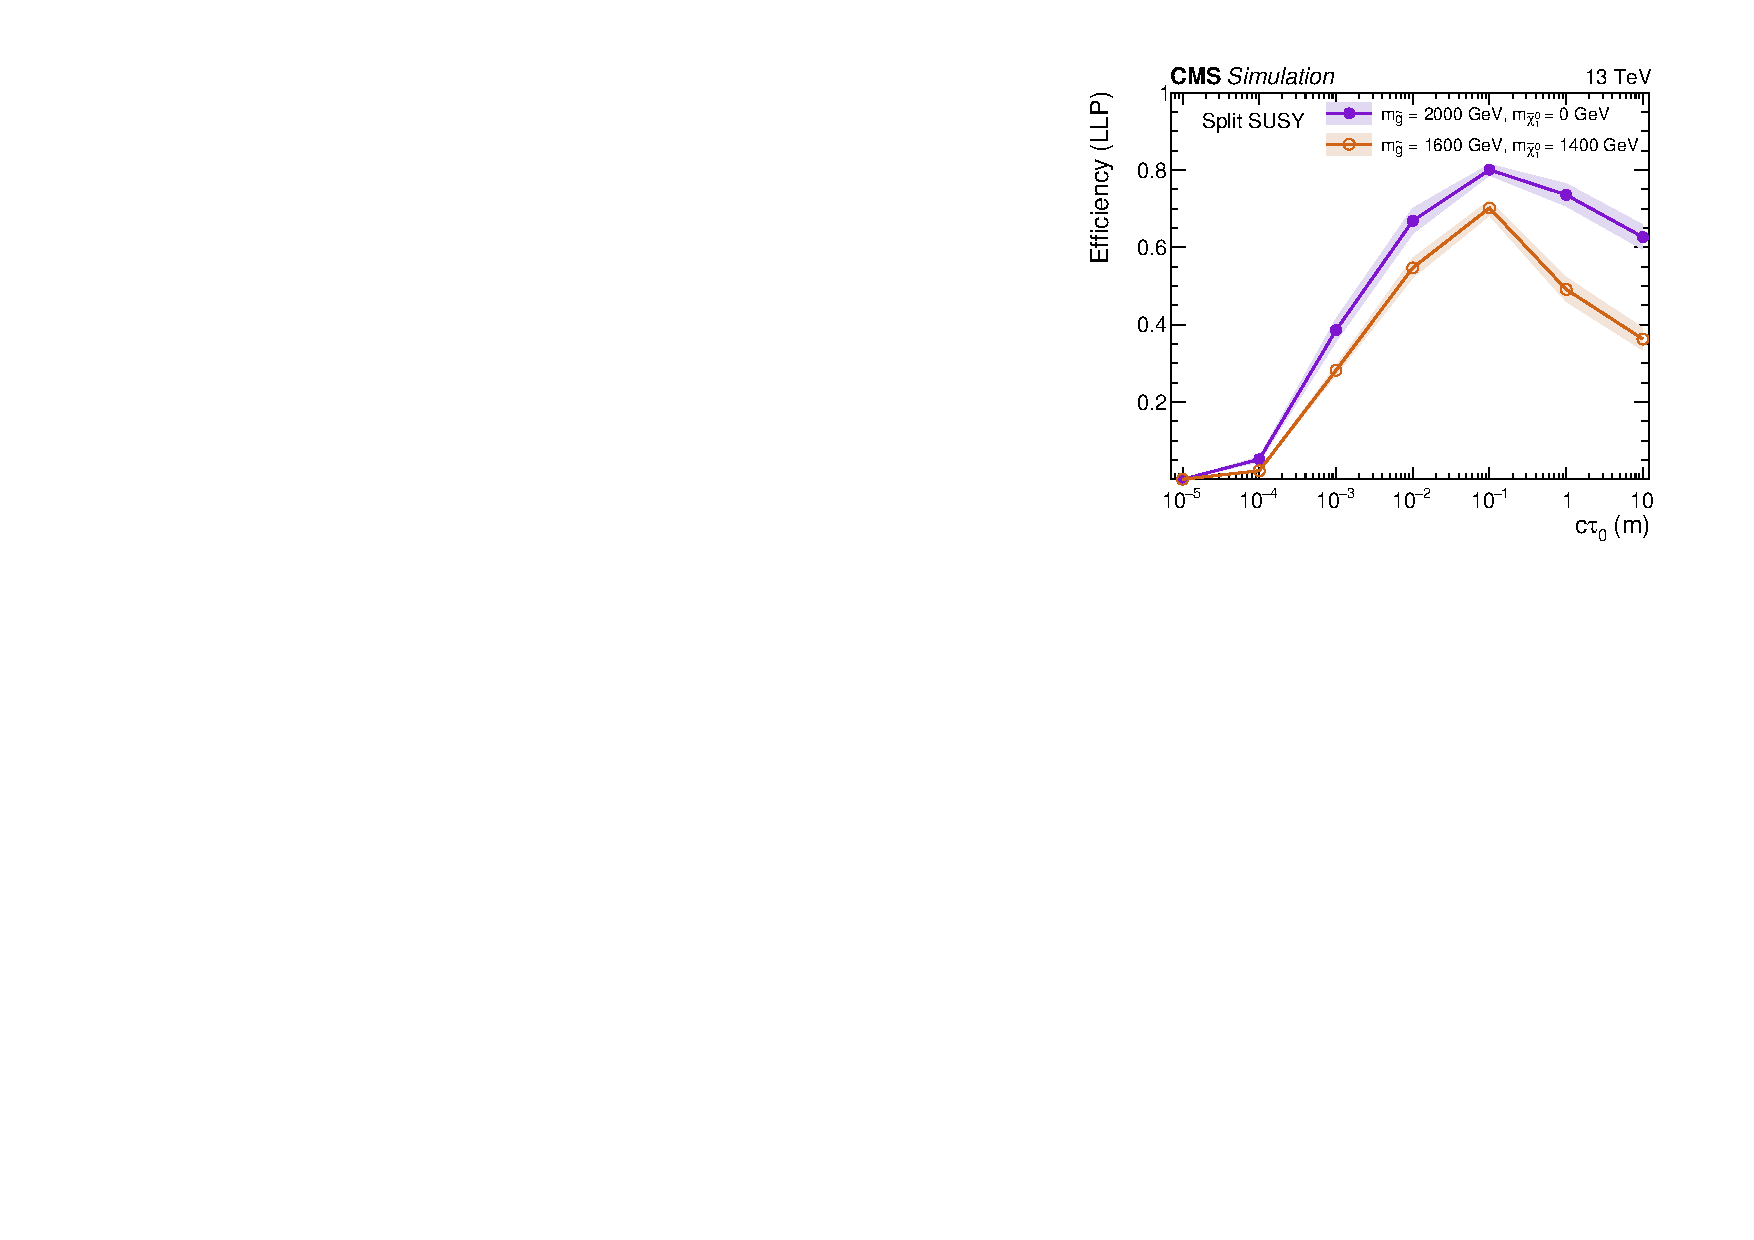
\includegraphics[width=0.48\textwidth]{figs/ctau.pdf}\hspace{0.03\textwidth}
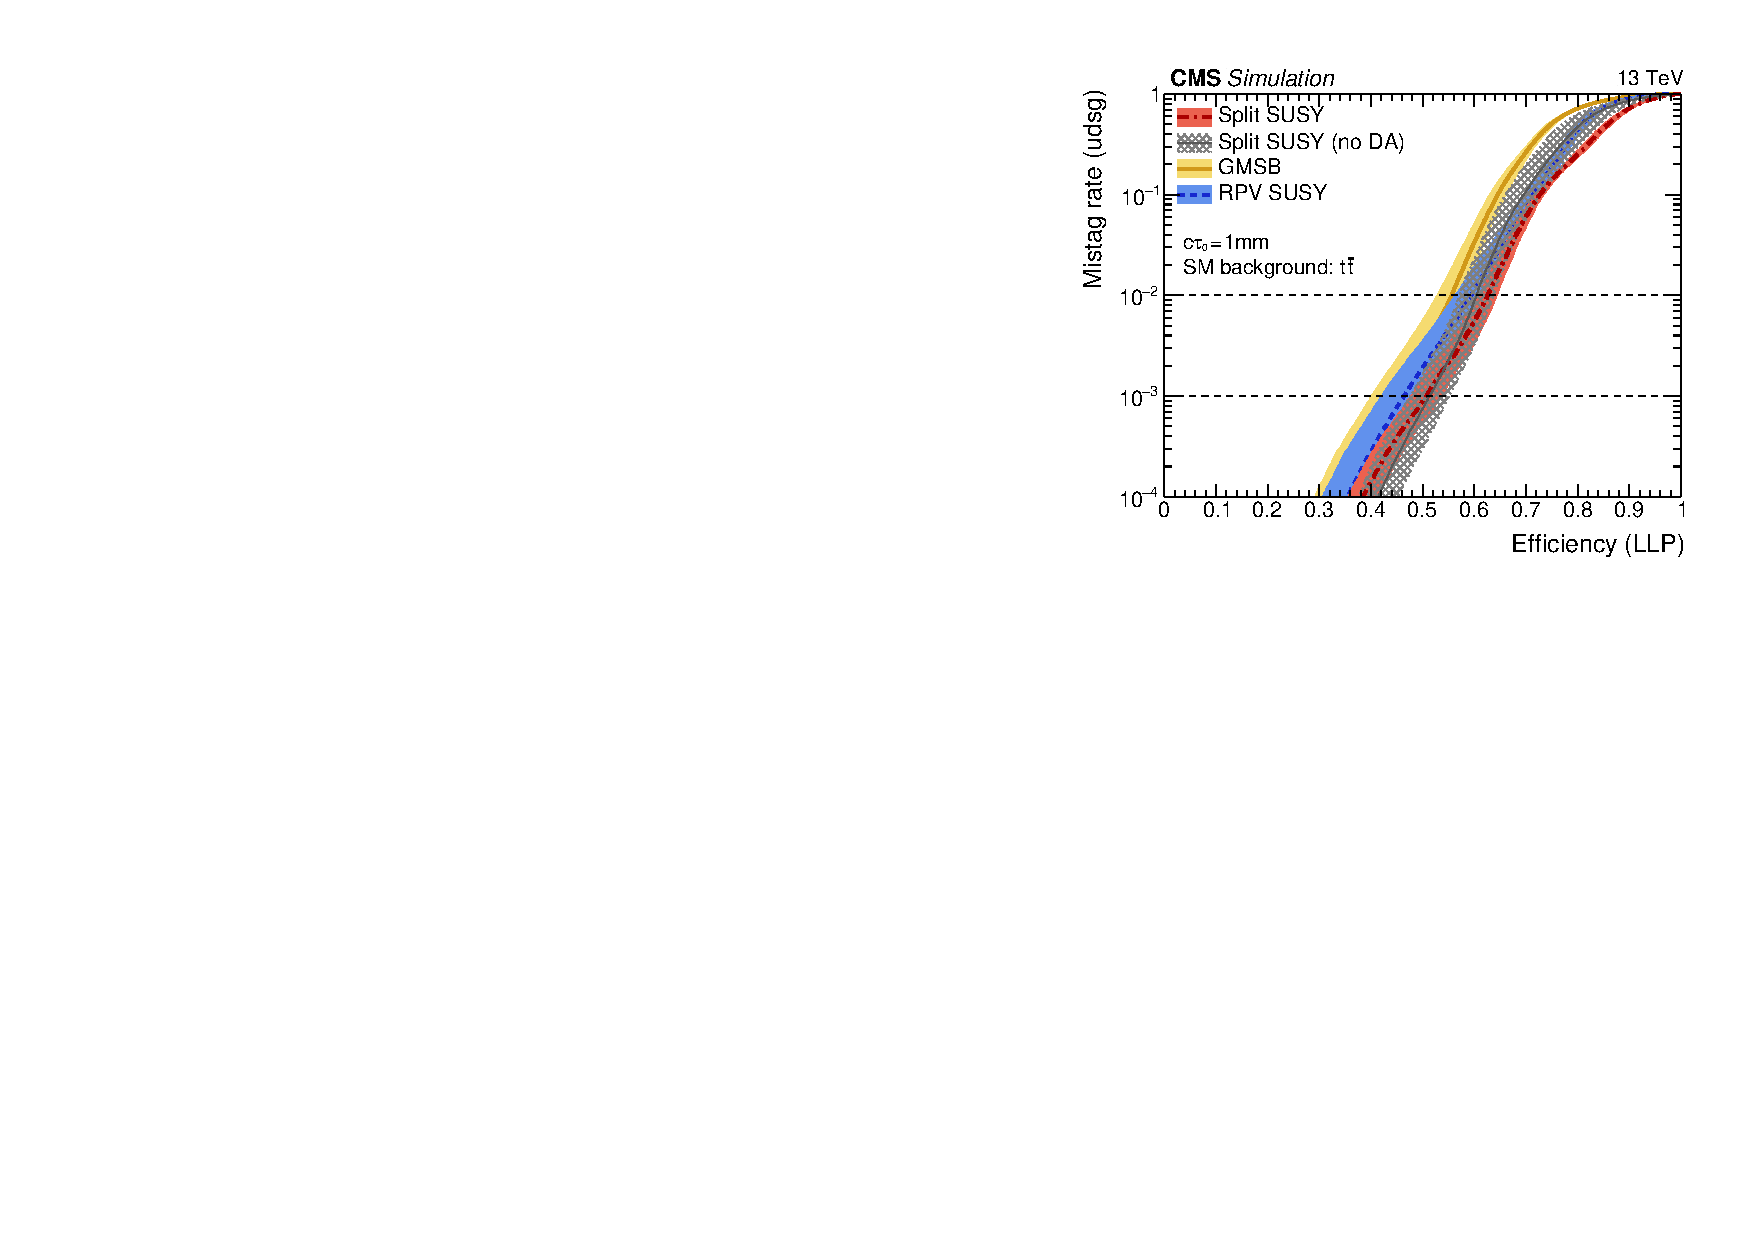
\includegraphics[width=0.48\textwidth]{figs/roc_1.pdf}
\centering
\caption{The figures are taken from Ref.~\cite{CMS-EXO-19-011}.}
\label{fig-3}
\end{figure*}

\section{Showcase search for long-lived gluinos}

\begin{figure*}[!ht]
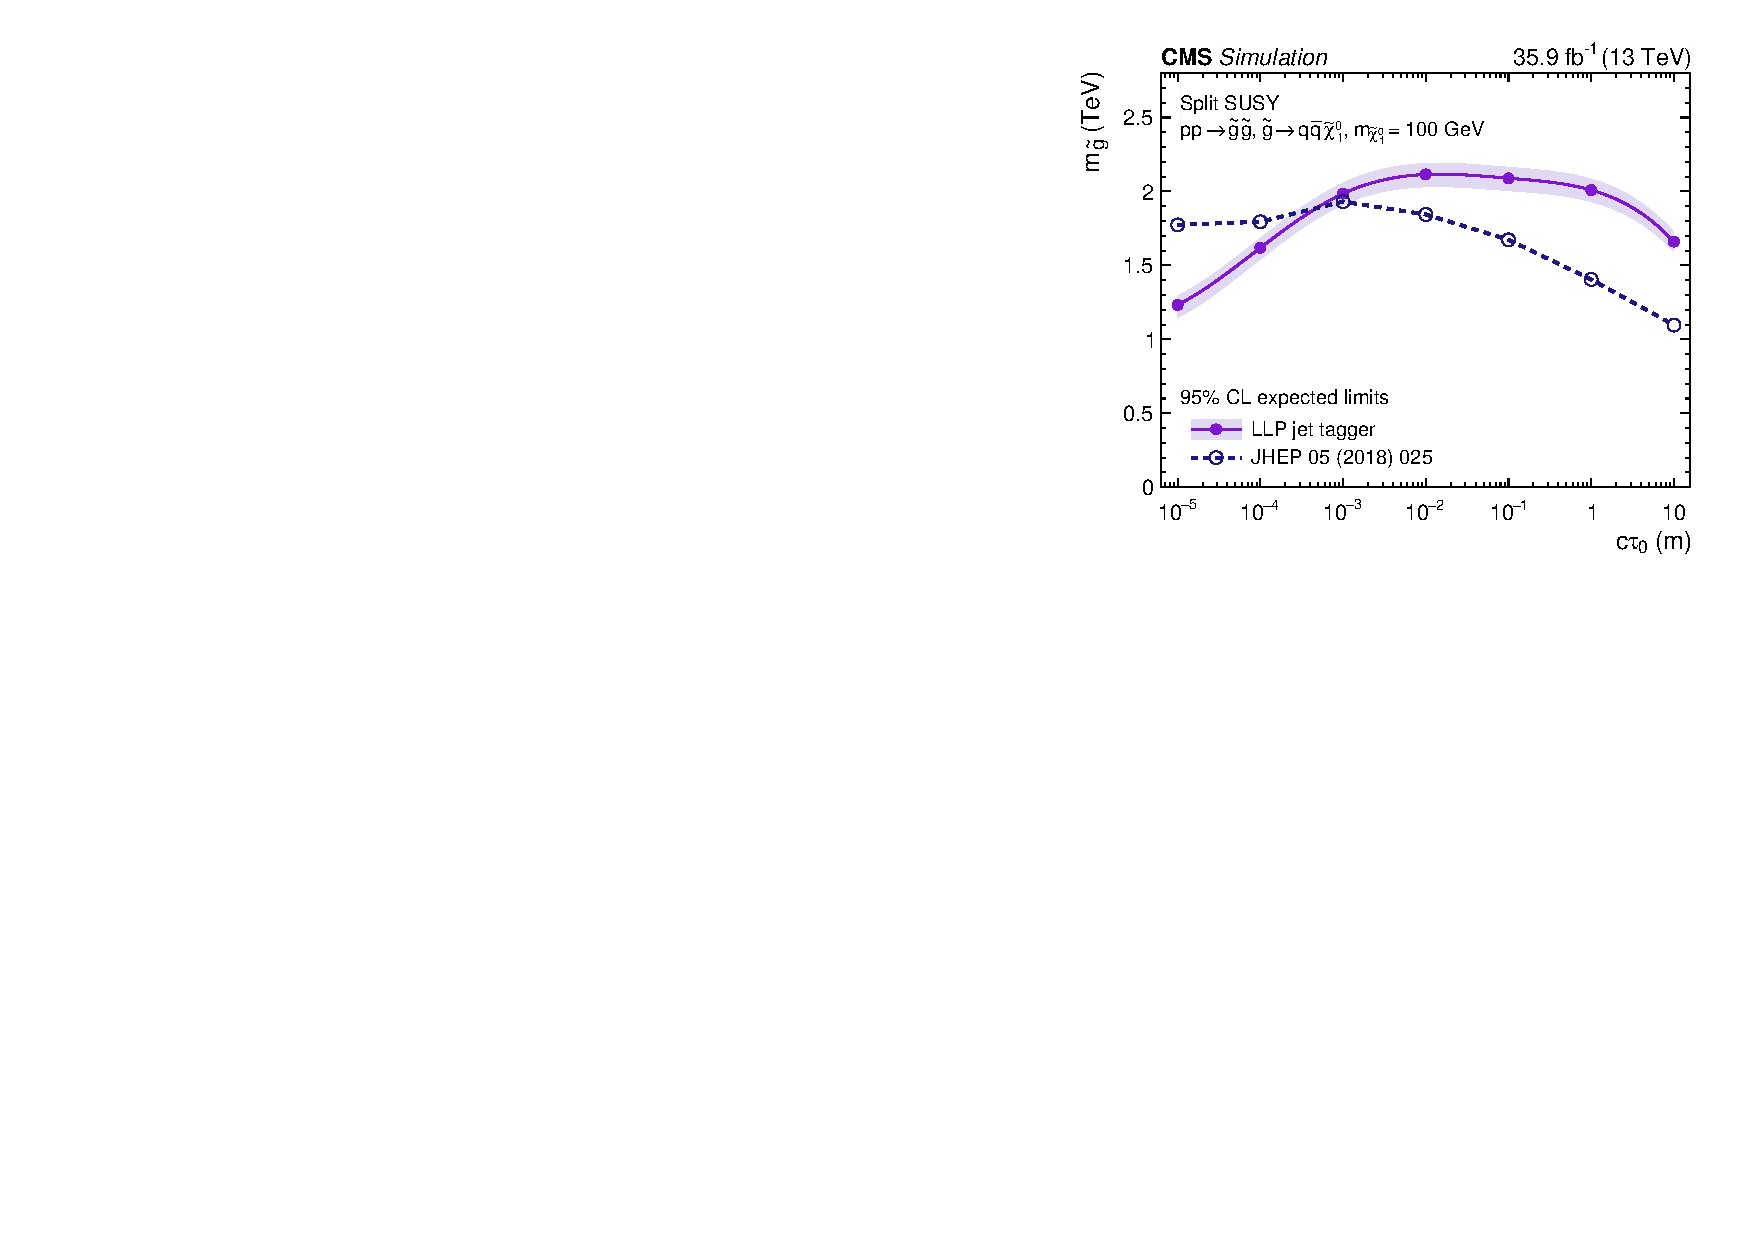
\includegraphics[width=0.48\textwidth]{figs/summaryU.pdf}\hspace{0.03\textwidth}
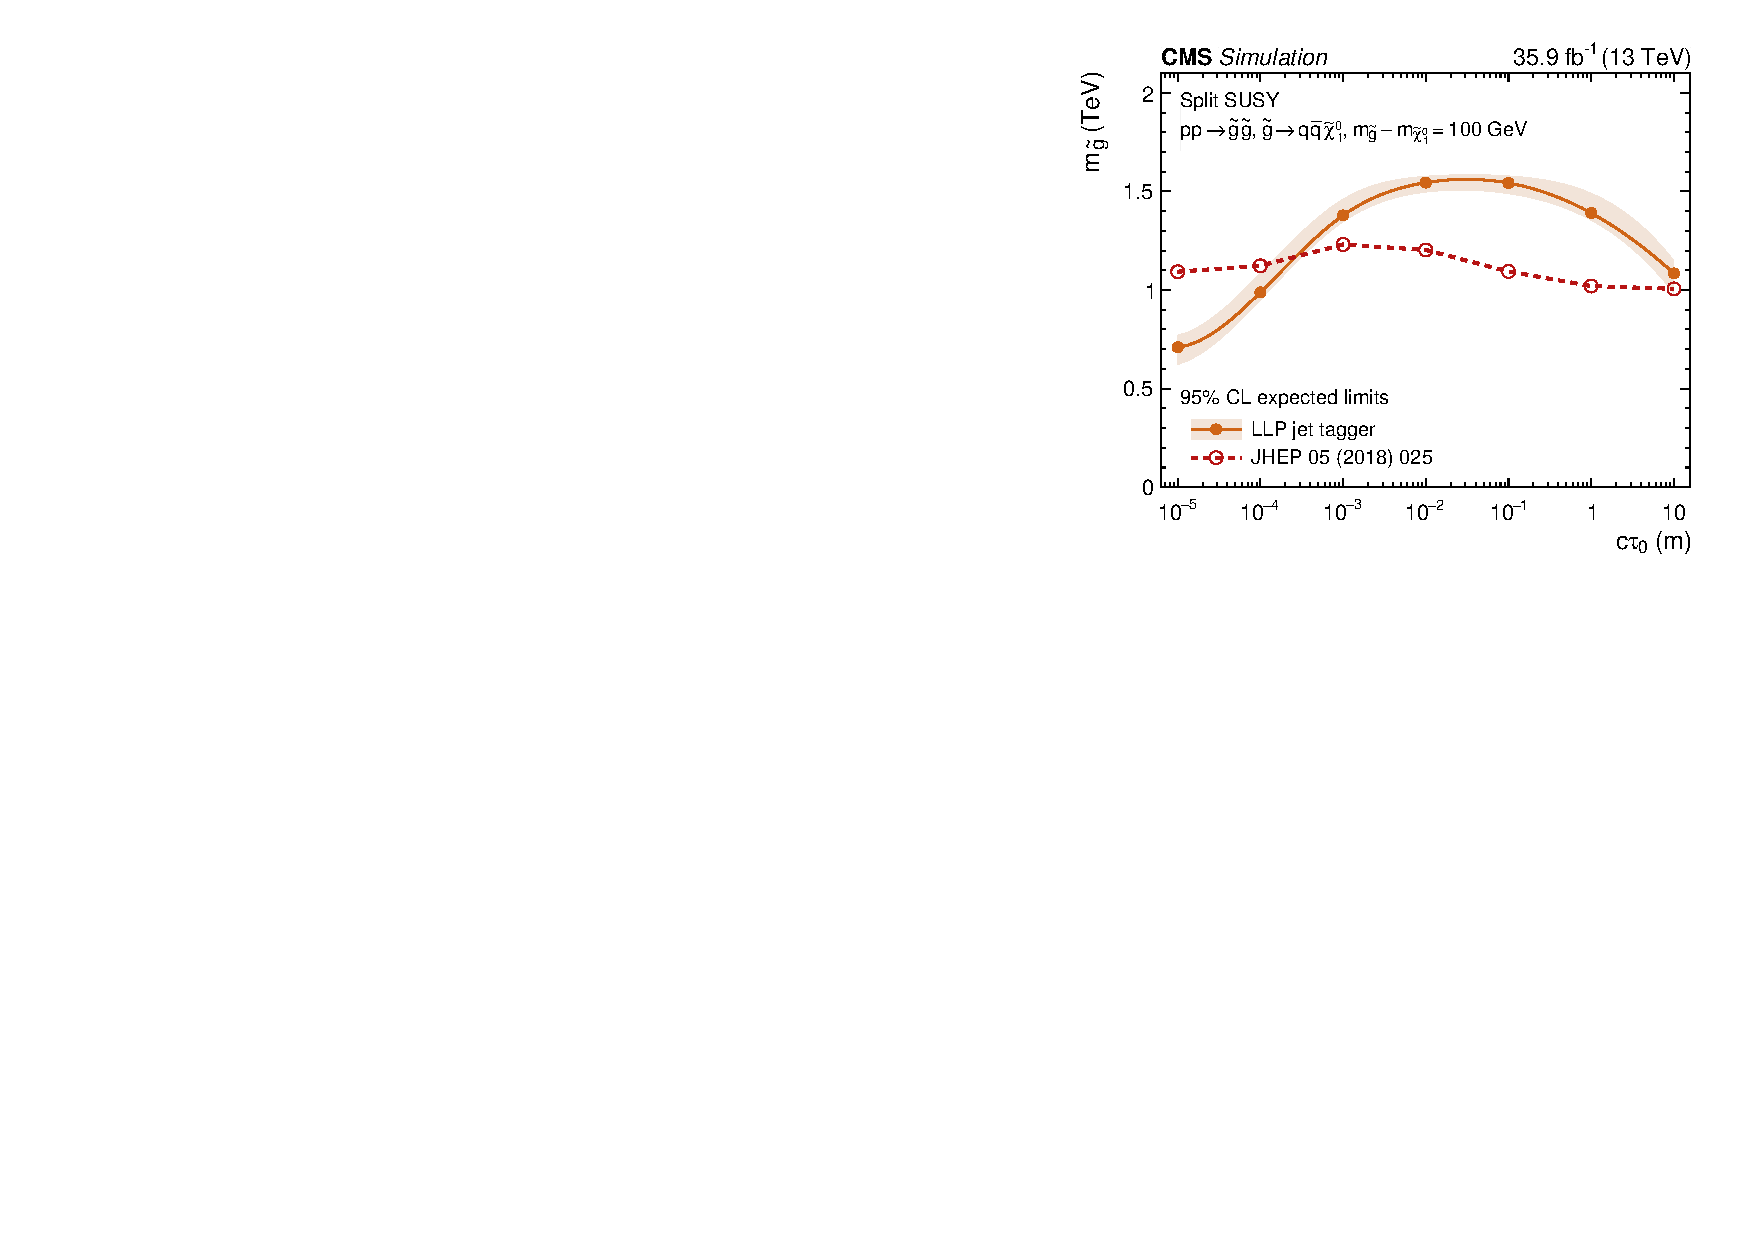
\includegraphics[width=0.48\textwidth]{figs/summaryC.pdf}
\centering
\caption{The figures are taken from Ref.~\cite{CMS-EXO-19-011}.}
\label{fig-4}
\end{figure*}

\clearpage

\begin{thebibliography}{}
\bibitem{ml-white-paper} Kim Albertsson et al., J. Phys. Conf. Ser. \textbf{1085} (2018), 022008, \href{http://www.arxiv.org/abs/1807.02876}{arXiv:1807.02876}
\bibitem{atlas} ATLAS Collaboration, JINST \textbf{3} (2008) S08003, \href{http://dx.doi.org/10.1088/1748-0221/3/08/S08003}{doi:10.1088/1748-0221/3/08/S08003}
\bibitem{cms}  CMS Collaboration, JINST \textbf{3} (2008) S08004,
\href{http://dx.doi.org/10.1088/1748-0221/3/08/S08004}{doi:10.1088/1748-0221/3/08/S08004}
\bibitem{batlas} ATLAS Collaboration, Eur. Phys. J. C \textbf{79} (2019) 970, \href{http://dx.doi.org/10.1140/epjc/s10052-019-7450-8}{doi:10.1140/epjc/s10052-019-7450-8}
\bibitem{bcms} CMS Collaboration, JINST \textbf{13} (2018) P05011,
\href{http://dx.doi.org/10.1088/1748-0221/13/05/P05011}{doi:10.1088/1748-0221/13/05/P05011}

\bibitem{CMS-EXO-19-011} CMS Collaboration, \textit{Submitted to MLST}, (2019), \href{https://arxiv.org/abs/1912.12238}{arXiv:1912.12238}



\end{thebibliography}

\end{document}
